\documentclass[letterpaper]{article} % DO NOT CHANGE THIS
\usepackage[submission]{aaai2027}  % DO NOT CHANGE THIS
\usepackage[hyphens]{url}  % DO NOT CHANGE THIS
\usepackage{graphicx} % DO NOT CHANGE THIS
\urlstyle{rm} % DO NOT CHANGE THIS
\def\UrlFont{\rm}  % DO NOT CHANGE THIS
\usepackage{natbib}  % DO NOT CHANGE THIS AND DO NOT ADD ANY OPTIONS TO IT
\usepackage{caption} % DO NOT CHANGE THIS AND DO NOT ADD ANY OPTIONS TO IT
\frenchspacing  % DO NOT CHANGE THIS
\usepackage{booktabs}
\pdfinfo{
/TemplateVersion (2027.1)
}
\setcounter{secnumdepth}{0}

% Notation used throughout.
\newcommand{\cotwo}{CO\textsubscript{2}}
\newcommand{\eurm}{\texteuro/m\textsuperscript{2}}
\newcommand{\kgm}{kg/m\textsuperscript{2}}

% Number sourcing convention (see README.md): every number carries a comment
% naming its source. "<split>/summary.csv <label> <column>" means
% control/results/analysis/<split>/summary.csv, row <label>, column <column>,
% rounded from full precision (2 decimals for EUR/m2 and kg/m2, 1 for hours,
% whole percent for ratios). REPORT.md means docs/REPORT.md at this commit.

\title{Tune the Baseline, Check the Objective: A Pre-Registered Evaluation\\of Residual RL for Greenhouse Climate Control}
\author{Anonymous Submission}
\affiliations{}

\begin{document}

\maketitle

\begin{abstract}
% 60-day seasons and the three 2012 test cities: REPORT.md Sec. 2.1 and Sec. 2.6.
Reinforcement learning (RL) for greenhouse climate control has been reported against a rule-based controller left at its default setpoints, and scored by a profit objective that trades fruit revenue against the cost of heating, lighting and \cotwo{}. We test both choices in the GreenLight-Gym tomato simulator under a pre-registered protocol: each experiment's arms, seeds and decision rule were recorded before it ran, and 2012 weather for Amsterdam, London and Abbotsford was scored once.
% 12 setpoints, 200 trials: REPORT.md Sec. 2.3 (E1, registered-b89a61b1).
% 73 to 76%: share = -g(rb_default) / (-g(rb_default) + g(ppo)), g = <split>/summary.csv profit_gain_iqm;
% amsterdam 7.4258/(7.4258+2.7354) = 0.7308; london 6.4689/(6.4689+2.0797) = 0.7567; abbotsford 9.2030/(9.2030+3.2529) = 0.7388.
Tuning the rule controller's 12 setpoints with 200 trials of an off-the-shelf Bayesian optimizer (TPE) recovers about three quarters (73 to 76\%) of PPO's profit lead over the default rules on each test split.
% 28 to 32%: 1 - ppo/rb_tuned yield_kg_m2_iqm per split: amsterdam 0.3066, london 0.2792, abbotsford 0.3183.
PPO's remaining lead comes with 28 to 32\% less fruit growth than the tuned rules, and a controller that switches every actuator off earns the highest 60-day profit on every split.
% 0.15: REPORT.md Sec. 2.4. 0.30 to 0.54: <split>/summary.csv residual_w05 profit_gain_iqm (0.3044, 0.3958, 0.5399).
% 20 to 25%: 1 - residual_w05/rb_tuned viol_hours_sum_iqm: amsterdam 1-292.5625/365.1875 = 0.1989; london 1-343.06875/456.9375 = 0.2492; abbotsford 1-444.31875/559.8125 = 0.2063.
A residual PPO agent that moves each control by at most 0.15 of its [0, 1] range from the tuned rules gains 0.30 to 0.54~\eurm{} per season over them with 20 to 25\% fewer violation hours, and passes its pre-registered decision rule on all three splits; its PID-Lagrangian constrained variant, on which our headline was registered, fails its violation-hour criterion in Amsterdam. We also report two bugs in the simulator's reward. On this benchmark, profit alone ranks doing nothing first: a fair comparison needs a baseline tuned with stated effort and guards on both the climate and the crop.
\end{abstract}

\section{Introduction}

% GreenLight-Gym's baseline (fixed grower setpoints, untuned; PPO outperforms it; the authors note that tuning the rules would
% give a more competitive baseline): arXiv 2410.05336v2, paraphrased, checked by the orchestrator for issue 66.
% 15 minutes: the simulator's 900 s control step, REPORT.md Sec. 2.1.
A greenhouse with supplemental lighting buys heat, electricity and \cotwo{} to grow a crop, and its climate controller decides every 15 minutes how much of each to use while keeping \cotwo{}, air temperature and humidity inside safe ranges. RL is a natural candidate for this control problem, and process simulators let it be tested before a grower takes any risk. GreenLight-Gym \cite{vanlaatum2025greenlightgym} wraps the GreenLight greenhouse model \cite{katzin2020greenlight} as an RL environment and reports PPO outperforming a rule-based controller with fixed grower setpoints, noting that tuning those rules would give a more competitive baseline. We measure how much. Building energy control has similar benchmarks \cite{blum2021boptest,jimenezraboso2021sinergym,vazquezcanteli2019citylearn} and reviews \cite{wang2020buildingrl,nagy2023tenquestions}.

Two choices decide what a reported gain means. The first is the baseline: a learned controller compared with untuned rules gets credit for any improvement that tuning the rules would also have found. The second is the objective: a gain in profit means a better controller only if profit rewards running the greenhouse well. We test both, and then ask whether a residual agent, which keeps the rules as its default and learns a bounded correction, adds to a tuned rule controller. Our contributions:
\begin{itemize}
% 200 trials, 12 setpoints: REPORT.md Sec. 2.3. 73 to 76%: see abstract comment.
\item \emph{A tuned baseline.} Under the protocol's effort budget (200 TPE trials for the rules; GreenLight-Gym's hyperparameters, untuned, for PPO), tuning the rule controller's 12 setpoints recovers 73 to 76\% of PPO's profit lead over the default rules on each of three held-out 2012 test splits (Figure~\ref{fig:main}a).
% 28 to 32%: see abstract comment.
\item \emph{An objective check.} PPO's remaining lead comes with 28 to 32\% less fruit growth than the tuned rules, and a controller with every actuator off earns the highest 60-day profit on every split: the objective rewards not operating (Figure~\ref{fig:main}b).
% 0.30 to 0.54 and 20 to 25%: see abstract comment.
\item \emph{A residual agent on tuned rules.} A residual PPO agent gains 0.30 to 0.54~\eurm{} per season over the tuned rules with 20 to 25\% fewer violation hours and passes its registered rule on all three splits; the PID-Lagrangian constrained variant fails its violation-hour criterion in Amsterdam.
\item \emph{Two reward bugs} in the simulator: its lamp penalty never fires, and its \cotwo{} and temperature penalty labels are swapped.
\item \emph{A protocol} with decision rules registered before each run, an append-only ledger and a test set opened once.
\end{itemize}

\section{Related Work}

% SafeGreenRL facts (5 seeds, Amsterdam 2008 to 2011 training, Amsterdam and London 2012 tests, price and parameter shifts) and
% Bie et al. facts (residual PPO bounded at +-0.15 on the untuned rule controller): from the issue-66 brief's verified reference notes, not REPORT.md.
Closest to us, SafeGreenRL \cite{sharma2026safegreenrl} compares PPO-Lagrangian with profit-only and fixed-penalty PPO on GreenLight-Gym2 over 5 seeds, training on Amsterdam 2008 to 2011 and testing on Amsterdam and London 2012 and under price and parameter shifts; PPO-Lagrangian met its budget at lower profit. \citet{bie2026calibration} audit reward components and use a residual PPO, bounded at $\pm 0.15$, on the official, untuned rule controller with a fixed reward mixture. Unlike \citet{bie2026calibration}, we tune the rule controller with a stated effort; we also peg constraint budgets to that tuned controller, register decision rules before each run with a single-use test set, and check whether the evaluation metric, profit, ranks a do-nothing controller first. Greenhouse climate control has also been approached with model predictive control, alone or combined with RL \cite{morcego2023rlmpc,mallick2025rlmpc,msaad2025rlguided}, and with other AI methods \cite{hemming2019remote,hemming2020cherry,cao2022igrow,liu2025greenhouse}. Our agent builds on residual policy learning \cite{silver2018residual,johannink2019residual} and PID-Lagrangian multipliers \cite{stooke2020pid}. Our statistics follow \citet{agarwal2021precipice} and wider guidance on RL evaluation \cite{henderson2018matters,engstrom2020implementation,patterson2024empirical}, and our registrations follow the logic of preregistration \cite{nosek2018preregistration}. An objective that pays a controller for not operating is a case of the misspecification studied as specification gaming and reward hacking \cite{krakovna2020specgaming,skalse2022reward,amodei2016concrete}.

\section{Setup}

\begin{table*}[t]
\centering
\small
\setlength{\tabcolsep}{3.5pt}
\begin{tabular}{lr@{\ }lr@{\ }lrrrrr@{\ }l}
\toprule
 & \multicolumn{2}{c}{Profit (\eurm{})} & \multicolumn{2}{c}{Gain over tuned rules (\eurm{})} & \multicolumn{4}{c}{Violation hours (h)} & \multicolumn{2}{c}{Fruit growth (\kgm{})} \\
\cmidrule(lr){2-3}\cmidrule(lr){4-5}\cmidrule(lr){6-9}\cmidrule(lr){10-11}
Controller & IQM & [95\% CI] & IQM & [95\% CI] & \cotwo{} & Temp. & RH & $\Sigma$ & IQM & [95\% CI] \\
\midrule
% Generated from the three test summary.csv files; each row's comment names file, label, n_runs, invalid_episodes and the columns in order.
\multicolumn{11}{l}{\emph{Amsterdam 2012}} \\
% amsterdam_2012/summary.csv rb_default (n_runs=1, invalid_episodes=0): profit_eur_m2_iqm, profit_gain_iqm, viol_hours_co2/temp/rh_iqm, viol_hours_sum_iqm, yield_kg_m2_iqm
Default rules & $-9.34$ &  & $-7.43$ &  & 0.0 & 95.8 & 666.1 & 761.9 & 10.98 &  \\
% amsterdam_2012/summary.csv rb_tuned (n_runs=1, invalid_episodes=0): profit_eur_m2_iqm, viol_hours_co2/temp/rh_iqm, viol_hours_sum_iqm, yield_kg_m2_iqm (gain is the reference, 0 by definition)
Tuned rules & $-1.92$ &  & ref. &  & 0.0 & 83.1 & 282.1 & 365.2 & 8.59 &  \\
% amsterdam_2012/summary.csv ppo (n_runs=5, invalid_episodes=0): profit_eur_m2_iqm/_lo/_hi, profit_gain_iqm/_lo/_hi, viol_hours_co2/temp/rh_iqm, viol_hours_sum_iqm, yield_kg_m2_iqm/_lo/_hi
PPO & 0.80 & [0.74, 0.86] & 2.74 & [2.69, 2.78] & 0.0 & 117.0 & 143.8 & 260.8 & 5.96 & [5.93, 5.98] \\
% amsterdam_2012/summary.csv residual_w05 (n_runs=10, invalid_episodes=0): profit_eur_m2_iqm/_lo/_hi, profit_gain_iqm/_lo/_hi, viol_hours_co2/temp/rh_iqm, viol_hours_sum_iqm, yield_kg_m2_iqm/_lo/_hi
Residual (fixed penalty) & $-1.64$ & [$-1.69$, $-1.58$] & 0.30 & [0.25, 0.35] & 0.0 & 49.0 & 243.6 & 292.6 & 8.77 & [8.75, 8.78] \\
% amsterdam_2012/summary.csv lag_b100 (n_runs=10, invalid_episodes=0): profit_eur_m2_iqm/_lo/_hi, profit_gain_iqm/_lo/_hi, viol_hours_co2/temp/rh_iqm, viol_hours_sum_iqm, yield_kg_m2_iqm/_lo/_hi
Residual (constrained) & $-1.51$ & [$-1.56$, $-1.46$] & 0.38 & [0.35, 0.42] & 0.0 & 75.1 & 324.8 & 399.9$^\dagger$ & 8.76 & [8.74, 8.78] \\
% amsterdam_2012/summary.csv zero_controls (n_runs=1, invalid_episodes=0): profit_eur_m2_iqm, profit_gain_iqm, viol_hours_co2/temp/rh_iqm, viol_hours_sum_iqm, yield_kg_m2_iqm
All off & 3.10 &  & 5.02 &  & 556.4 & 999.2 & 1421.9 & 2977.5 & 1.94 &  \\
\midrule
\multicolumn{11}{l}{\emph{London 2012}} \\
% london_2012/summary.csv rb_default (n_runs=1, invalid_episodes=0): profit_eur_m2_iqm, profit_gain_iqm, viol_hours_co2/temp/rh_iqm, viol_hours_sum_iqm, yield_kg_m2_iqm
Default rules & $-6.56$ &  & $-6.47$ &  & 0.0 & 97.4 & 668.9 & 766.4 & 11.00 &  \\
% london_2012/summary.csv rb_tuned (n_runs=1, invalid_episodes=0): profit_eur_m2_iqm, viol_hours_co2/temp/rh_iqm, viol_hours_sum_iqm, yield_kg_m2_iqm (gain is the reference)
Tuned rules & $-0.09$ &  & ref. &  & 0.0 & 86.4 & 370.5 & 456.9 & 8.89 &  \\
% london_2012/summary.csv ppo (n_runs=5, invalid_episodes=0): profit_eur_m2_iqm/_lo/_hi, profit_gain_iqm/_lo/_hi, viol_hours_co2/temp/rh_iqm, viol_hours_sum_iqm, yield_kg_m2_iqm/_lo/_hi
PPO & 1.90 & [1.84, 1.96] & 2.08 & [2.02, 2.14] & 0.0 & 85.3 & 154.0 & 239.2 & 6.41 & [6.39, 6.43] \\
% london_2012/summary.csv residual_w05 (n_runs=10, invalid_episodes=0): profit_eur_m2_iqm/_lo/_hi, profit_gain_iqm/_lo/_hi, viol_hours_co2/temp/rh_iqm, viol_hours_sum_iqm, yield_kg_m2_iqm/_lo/_hi
Residual (fixed penalty) & 0.25 & [0.20, 0.30] & 0.40 & [0.35, 0.44] & 0.0 & 44.1 & 299.0 & 343.1 & 9.15 & [9.14, 9.17] \\
% london_2012/summary.csv lag_b100 (n_runs=10, invalid_episodes=0): profit_eur_m2_iqm/_lo/_hi, profit_gain_iqm/_lo/_hi, viol_hours_co2/temp/rh_iqm, viol_hours_sum_iqm, yield_kg_m2_iqm/_lo/_hi
Residual (constrained) & 0.38 & [0.35, 0.41] & 0.46 & [0.43, 0.49] & 0.0 & 68.1 & 376.1 & 444.2 & 9.13 & [9.11, 9.15] \\
% london_2012/summary.csv zero_controls (n_runs=1, invalid_episodes=0): profit_eur_m2_iqm, profit_gain_iqm, viol_hours_co2/temp/rh_iqm, viol_hours_sum_iqm, yield_kg_m2_iqm
All off & 3.21 &  & 3.31 &  & 760.1 & 912.8 & 1385.8 & 3058.7 & 2.01 &  \\
\midrule
\multicolumn{11}{l}{\emph{Abbotsford 2012}} \\
% abbotsford_2012/summary.csv rb_default (n_runs=1, invalid_episodes=0): profit_eur_m2_iqm, profit_gain_iqm, viol_hours_co2/temp/rh_iqm, viol_hours_sum_iqm, yield_kg_m2_iqm
Default rules & $-12.52$ &  & $-9.20$ &  & 0.0 & 95.3 & 828.0 & 923.3 & 11.34 &  \\
% abbotsford_2012/summary.csv rb_tuned (n_runs=1, invalid_episodes=0): profit_eur_m2_iqm, viol_hours_co2/temp/rh_iqm, viol_hours_sum_iqm, yield_kg_m2_iqm (gain is the reference)
Tuned rules & $-3.32$ &  & ref. &  & 0.0 & 140.8 & 419.1 & 559.8 & 8.28 &  \\
% abbotsford_2012/summary.csv ppo (n_runs=5, invalid_episodes=0): profit_eur_m2_iqm/_lo/_hi, profit_gain_iqm/_lo/_hi, viol_hours_co2/temp/rh_iqm, viol_hours_sum_iqm, yield_kg_m2_iqm/_lo/_hi
PPO & $-0.06$ & [$-0.14$, 0.01] & 3.25 & [3.18, 3.33] & 0.0 & 37.2 & 195.6 & 232.8 & 5.65 & [5.62, 5.67] \\
% abbotsford_2012/summary.csv residual_w05 (n_runs=10, invalid_episodes=0): profit_eur_m2_iqm/_lo/_hi, profit_gain_iqm/_lo/_hi, viol_hours_co2/temp/rh_iqm, viol_hours_sum_iqm, yield_kg_m2_iqm/_lo/_hi
Residual (fixed penalty) & $-2.80$ & [$-2.86$, $-2.73$] & 0.54 & [0.47, 0.61] & 0.1 & 85.4 & 358.8 & 444.3 & 8.42 & [8.41, 8.44] \\
% abbotsford_2012/summary.csv lag_b100 (n_runs=10, invalid_episodes=0): profit_eur_m2_iqm/_lo/_hi, profit_gain_iqm/_lo/_hi, viol_hours_co2/temp/rh_iqm, viol_hours_sum_iqm, yield_kg_m2_iqm/_lo/_hi
Residual (constrained) & $-2.66$ & [$-2.70$, $-2.60$] & 0.63 & [0.59, 0.67] & 0.0 & 117.3 & 434.1 & 551.5 & 8.43 & [8.40, 8.45] \\
% abbotsford_2012/summary.csv zero_controls (n_runs=1, invalid_episodes=0): profit_eur_m2_iqm, profit_gain_iqm, viol_hours_co2/temp/rh_iqm, viol_hours_sum_iqm, yield_kg_m2_iqm
All off & 1.91 &  & 5.29 &  & 700.2 & 939.1 & 1373.9 & 3013.1 & 1.19 &  \\
\bottomrule
\end{tabular}
% Seed counts: n_runs column of each summary.csv (ppo 5; residual_w05 10; lag_b100 10; baselines 1). Seasons per split: 8 (REPORT.md Sec. 2.6).
\caption{Results on the three 2012 test splits, each 8 seasons of 60 days. IQM [95\% stratified-bootstrap CI] over runs $\times$ seasons; PPO has 5 runs, each residual agent 10. The rules and All off are deterministic, one run per season, so their intervals are omitted. Gain is the IQM of the per-season profit difference from the tuned rules' same season. Hours are IQMs per constraint; $\Sigma$, their sum, is what the registered hour criterion, rule (b) in the Protocol paragraph, compares. $^\dagger$Above the tuned rules' $\Sigma$, so (b) fails.}
\label{tab:results}
\end{table*}

% Figure: figures/fig_main.pdf, drawn by figures/make_figure.py from the three test summary.csv files, which prints every plotted value.
% (a) tuning = -rb_default profit_gain_iqm (7.43, 6.47, 9.20), PPO = ppo profit_gain_iqm (2.74, 2.08, 3.25), share as in the abstract comment.
% (b) x = yield_kg_m2_iqm, y = profit_eur_m2_iqm for rb_default, rb_tuned, residual_w05, lag_b100, ppo, zero_controls on each split.
\begin{figure}[t]
\centering
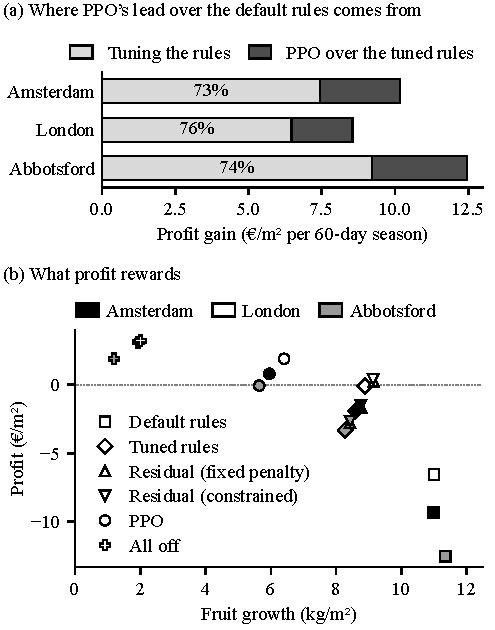
\includegraphics[width=\columnwidth]{figures/fig_main}
\caption{The 2012 test splits. (a) PPO's profit lead over the default rules, split into the tuned rules' gain over the default rules and PPO's gain over the tuned rules (paired-gain IQMs); the percentage is tuning's share. (b) Profit IQM against fruit-growth IQM per controller and split. All off and PPO earn the most and grow the least fruit. The tuned rules and both residual agents overlap at this scale; Table~\ref{tab:results} gives their values.}
\label{fig:main}
\end{figure}

\subsubsection{Simulator and metrics.}
% 60 days, 900 s steps, 5,760 steps, 6 controls, safe ranges, prices: REPORT.md Sec. 2.1 (docs/PROTOCOL.md Sec. 1).
We use the GreenLight-Gym tomato environment (the GreenLight-Gym2 code base), pinned to one commit; we call the GreenLight-Gym code and its defaults \emph{upstream}. A season is 60 days at 15-minute steps (5,760 steps). The controller sets six controls in $[0, 1]$: boiler, \cotwo{} dosing, thermal screen, roof vents, lamps and blackout screen. The safe ranges are 300 to 1600~ppm \cotwo{}, 15 to 34\,$^\circ$C air temperature and 50 to 85\% relative humidity (RH). Prices are upstream's fixed defaults (tomatoes 1.60\,\texteuro/kg fresh weight; heat 0.09\,\texteuro/kWh; electricity 0.30\,\texteuro/kWh; \cotwo{} 0.30\,\texteuro/kg). Our grader computes every metric from raw states and controls and never imports the reward code. Profit (\eurm{}, the primary metric) is fruit revenue minus heating, electricity and \cotwo{} costs over the season. For each of \cotwo{}, temperature and RH, violation hours are the season's hours (steps $\times$ 0.25~h) with that variable outside its range; a season has 1,440 hours. Fruit growth (\kgm{}, fresh weight) is the net change in standing fruit over the season, not harvested yield. Reading the simulator's source, we found two reward bugs: its lamp penalty never fires, and its \cotwo{} and temperature penalty labels are swapped. Our reward reports each cost under its true name, with a test of hand-computed values for each term. Upstream also catches solver errors and truncates the episode; we count such episodes as invalid and never drop them.

\subsubsection{Controllers.}
% 12 setpoints, TPE seed 0, 200 trials, 9 TRAIN_EVAL seasons: REPORT.md Sec. 2.3 and Sec. 2.6 (E1, registered-b89a61b1).
% gamma 0.9631, learning rate 2e-5, 2,000,000 steps: REPORT.md Sec. 2.3 (control/configs/ppo.yml).
% Upstream's reward = the fixed-penalty reward at w = 1, bit for bit: REPORT.md Sec. 2.4; PPO trains at w = 1 (train.py PENALTY_WEIGHT).
% "Upstream's return" = REPORT.md's paper return, the sum of upstream's per-step reward (REPORT.md Sec. 2.2).
% Three values each: w in {0.5, 1, 4} (REPORT.md Sec. 2.4, E4); budget multiplier b in {1.0, 0.5, 0.25} (REPORT.md Sec. 2.5, E5 and E5b).
The \emph{default rules} are upstream's rule-based controller with its default parameters. The \emph{tuned rules} are the same controller with its 12 setpoints tuned by Optuna's TPE sampler \cite{akiba2019optuna,bergstra2011tpe} (one study, seed 0, 200 trials) to maximize upstream's return, the season sum of upstream's reward, averaged over nine training seasons. \emph{PPO} \cite{schulman2017ppo} runs in Stable-Baselines3 \cite{raffin2021sb3} on upstream's reward (scaled profit minus the three violation costs, the fixed-penalty reward below at $w = 1$) with upstream's configuration unchanged (e.g.\ $\gamma = 0.9631$, learning rate $2 \times 10^{-5}$), since defaults are part of an RL result \cite{engstrom2020implementation}. This is the protocol's effort match: 200 tuning trials for the rules and none for PPO's hyperparameters; the residual agents' penalty weight and budget were each picked from three values on validation.
% 0.15, a in [-1,1]^6, w = 0.5 from {0.5, 1, 4}: REPORT.md Sec. 2.4 (E4, result-2a890455).
The \emph{residual agent} applies $u = \mathrm{clip}(u_{\mathrm{rb}} + 0.15\,a, 0, 1)$, where $u_{\mathrm{rb}}$ is the tuned rules' action and $a \in [-1, 1]^6$ the policy's, so each control moves at most 0.15 from the rules and a zero residual is exactly the tuned rules. With a \emph{fixed penalty}, its reward is scaled profit $- w\,(c_{\mathrm{CO_2}} + c_{\mathrm{T}} + c_{\mathrm{RH}})$, with $w = 0.5$ chosen from $\{0.5, 1, 4\}$ on validation.
% reward form, budget definition, zero CO2 budget, fixed multiplier 1 (PROTOCOL v2): REPORT.md Sec. 2.5.
% "14 of 15 runs": decision-c26a2bc9, quoted in REPORT.md Sec. 2.5.
The \emph{constrained variant} sets $w = 0$ and gives each constraint $i$ a PID-Lagrangian multiplier $\lambda_i$ \cite{stooke2020pid}, with reward $(r - \sum_i \lambda_i c_i)/(1 + \sum_i \lambda_i)$ and a budget equal to the tuned rules' mean per-step cost $c_i$ on the training seasons. The tuned rules never break the \cotwo{} range there, so that budget is 0; after a registered sweep in which $\lambda_{\mathrm{CO_2}}$ pinned at its cap in 14 of 15 runs, a protocol revision fixed the multiplier of a zero-budget constraint at 1. \emph{All off} sets every actuator to 0. Each learning arm trains for 2,000,000 steps.

\subsubsection{Splits.}
% Splits, start days, checkpoint interval 250,000: REPORT.md Sec. 2.6 and Sec. 3.2.
Training uses Amsterdam 2008, 2009 and 2011 with start days drawn from 45 to 75. Validation (Amsterdam 2010, start days 45, 59 and 75) selects checkpoints, saved every 250,000 steps, and decides every experiment. The test splits are 2012 seasons from eight start days (45 to 73, every 4 days) in Amsterdam, London and Abbotsford (British Columbia). Amsterdam's weather is the simulator's bundled data; London's and Abbotsford's come from the NASA POWER project (\url{power.larc.nasa.gov}).

\subsubsection{Protocol.}
% Registration, ledger, fingerprints: REPORT.md Sec. 3.1. IQM, stratified bootstrap, 2,000 replicates: REPORT.md Sec. 3.3.
Before its first run, each experiment was registered with its hypothesis, arms, seeds, metrics and decision rule as a row in an append-only ledger that records fingerprints of the scoring code and the protocol; later rows record runs, results and the decision to adopt or drop. Scores are interquartile means (IQM) over runs $\times$ seasons with 95\% percentile stratified-bootstrap confidence intervals (2,000 resamples) \cite{agarwal2021precipice}. $\Sigma$ denotes the sum of the three per-constraint hour IQMs; it has no CI. Sweeps used 5 seeds, and a configuration picked from a sweep was rerun on 10 fresh seeds before any claim \cite{patterson2024empirical}.
% Validation confirmations: validation/summary.csv "residual_w05 #36/f2fd" profit_gain_iqm/_lo/_hi = 0.4916 [0.4032, 0.5699];
% validation/summary.csv "lag_b100 #39/6d92" profit_gain_iqm/_lo/_hi = 0.5687 [0.5171, 0.6359].
The two residual agents were confirmed this way on validation, gaining 0.49 [0.40, 0.57] (fixed penalty) and 0.57 [0.52, 0.64]~\eurm{} (constrained) over the tuned rules' same seasons.
% Final rule (a), (b), (c), no 1.10 tolerance, headline on lag_b100: REPORT.md Sec. 5 (issue rule, final-registered-4d0a4ba9).
The test evaluation was registered with the selected checkpoints, and its rule, fixed before the run, applied per arm and split: an arm passes if (a) its profit CI lies entirely above the tuned rules' profit, (b) its $\Sigma$ hours are at or below the tuned rules' $\Sigma$, with no tolerance, and (c) it has no invalid episode or solver failure. The headline was registered as the constrained variant passing on all three splits. The test weather was then scored once; the scoring code refuses a second run.

\section{Results}

% invalid_episodes = 0 for every learning arm on every split (three test summary.csv files).
Table~\ref{tab:results} gives six controllers on each test split, and Figure~\ref{fig:main} draws two comparisons from it. No learning arm had an invalid episode. Two further scored arms, uniform random controls and PPO trained as upstream does on one 2010 season, are omitted from the table and figure for space.

\subsubsection{Tuning the baseline.}
% ppo_paper beats rb_default on every split (CI above, lower Sigma): REPORT.md Sec. 5.2 (descriptive, no rule registered for it in the final).
% 0.67 [0.56, 0.78]: amsterdam_2012/summary.csv ppo_paper profit_eur_m2_iqm/_lo/_hi; -9.34: rb_default profit_eur_m2_iqm.
% 253.8 vs 761.9: amsterdam_2012/summary.csv ppo_paper and rb_default viol_hours_sum_iqm.
The published comparison reproduces: PPO trained as upstream does, on one 2010 season, earns more than the default rules on every split, with a profit CI entirely above theirs and fewer $\Sigma$ hours (in Amsterdam, 0.67 [0.56, 0.78] against $-9.34$~\eurm{} and 253.8 against 761.9~h). The test registered no rule for this comparison, so it is descriptive.
% -7.43, -6.47, -9.20: <split>/summary.csv rb_default profit_gain_iqm. 2.74 [2.69, 2.78], 2.08 [2.02, 2.14], 3.25 [3.18, 3.33]: <split>/summary.csv ppo profit_gain_iqm/_lo/_hi.
On every split the tuned rules earn more than the default rules on the same seasons: the default rules' gain over the tuned rules is $-7.43$, $-6.47$ and $-9.20$~\eurm{} in Amsterdam, London and Abbotsford, while PPO's is 2.74 [2.69, 2.78], 2.08 [2.02, 2.14] and 3.25 [3.18, 3.33].
% 73%, 76%, 74%: see abstract comment. Validation 74%: validation/summary.csv rb_default profit_gain_iqm = -6.8965 and "ppo #33/0221" profit_gain_iqm = 2.3993; 6.8965/(6.8965+2.3993) = 0.7419.
Writing $G_{\mathrm{tune}}$ for the tuned rules' gain over the default rules and $G_{\mathrm{PPO}}$ for PPO's gain over the tuned rules, tuning accounts for $G_{\mathrm{tune}}/(G_{\mathrm{tune}} + G_{\mathrm{PPO}}) =$ 73\%, 76\% and 74\% of PPO's lead over the default rules (Figure~\ref{fig:main}a; 74\% on validation). This is a ratio of paired-gain IQMs: descriptive, with no CI.
% 8.59, 8.89, 8.28 vs 10.98, 11.00, 11.34: <split>/summary.csv rb_tuned and rb_default yield_kg_m2_iqm.
Tuning also lowered fruit growth, to 8.59, 8.89 and 8.28 from 10.98, 11.00 and 11.34~\kgm{}.

\subsubsection{What the objective rewards.}
% 5.96, 6.41, 5.65: <split>/summary.csv ppo yield_kg_m2_iqm; 8.59, 8.89, 8.28: rb_tuned yield_kg_m2_iqm; 31%, 28%, 32% = 1 - ratio (0.3066, 0.2792, 0.3183).
PPO's remaining lead comes from spending less, not from growing more. Its fruit growth is 5.96, 6.41 and 5.65~\kgm{} against the tuned rules' 8.59, 8.89 and 8.28, that is 31\%, 28\% and 32\% less (one minus the ratio of IQMs; no CI).
% Replay counts (seed 0, 24 test seasons, all but the first hour): REPORT.md Sec. 5.2, counted from the final's replay files (seed 0 only).
In the hourly replays of PPO's seed 0, \cotwo{} dosing, the lamps and the blackout screen stay at 0 in every hour but the first of each of its 24 test seasons.
% 3.10, 3.21, 1.91 and 2977.5, 3058.7, 3013.1 and 1.94, 2.01, 1.19: <split>/summary.csv zero_controls profit_eur_m2_iqm, viol_hours_sum_iqm, yield_kg_m2_iqm.
% Highest of all 8 labels per split (zero_controls, random, rb_default, rb_tuned, ppo_paper, ppo, residual_w05, lag_b100): checked on profit_eur_m2_iqm in each summary.csv.
% 0.80, 1.90, -0.06: <split>/summary.csv ppo profit_eur_m2_iqm.
All off takes this to its limit (Figure~\ref{fig:main}b): it earns the highest profit of all eight controllers scored on every split, 3.10, 3.21 and 1.91~\eurm{} against PPO's 0.80, 1.90 and $-0.06$, with $\Sigma$ of 2977.5, 3058.7 and 3013.1~h (summed over the three constraints; a season has 1,440 hours) and fruit growth of 1.94, 2.01 and 1.19~\kgm{}. Over a 60-day window, profit pays for not operating. Only the violation-hour criterion keeps it out of a claim; nothing in the registered rule guards the crop.

\subsubsection{The residual agents.}
% 0.30 [0.25, 0.35], 0.40 [0.35, 0.44], 0.54 [0.47, 0.61]: <split>/summary.csv residual_w05 profit_gain_iqm/_lo/_hi.
% 292.6, 343.1, 444.3 vs 365.2, 456.9, 559.8: residual_w05 viol_hours_sum_iqm vs rb_tuned_viol_sum_iqm; 20%, 25%, 21% = 1 - ratio (0.1989, 0.2492, 0.2063).
% Fruit above: residual_w05 yield_kg_m2_iqm 8.77, 9.15, 8.42 vs rb_tuned 8.59, 8.89, 8.28.
% Pass/fail per part: REPORT.md Sec. 5.1 Tables 3 to 5, "Grade (#45's rule)" column (final-result-aee23915); (a) and (b) also readable from Table 1.
The fixed-penalty residual agent passes all three parts of the rule on every split. Its gains over the tuned rules' same seasons are 0.30 [0.25, 0.35], 0.40 [0.35, 0.44] and 0.54 [0.47, 0.61]~\eurm{}, its $\Sigma$ hours are 292.6, 343.1 and 444.3 against the rules' 365.2, 456.9 and 559.8 (20\%, 25\% and 21\% fewer), and its fruit growth is above the rules' on every split.
% Validation 0.49 [0.40, 0.57]: validation/summary.csv "residual_w05 #36/f2fd" profit_gain_iqm/_lo/_hi (0.4916 [0.4032, 0.5699]).
% Overlap: <split>/summary.csv residual_w05 profit_gain_lo/_hi: amsterdam [0.2524, 0.3535], hi < 0.4032; london [0.3500, 0.4381] and abbotsford [0.4674, 0.6055] overlap it.
Its Amsterdam CI lies below its validation CI, 0.49 [0.40, 0.57], without overlapping; London's and Abbotsford's overlap it.

% 0.38 [0.35, 0.42], 0.46 [0.43, 0.49], 0.63 [0.59, 0.67]: <split>/summary.csv lag_b100 profit_gain_iqm/_lo/_hi.
% CIs overlap: lag_b100 profit_gain_lo (0.3469, 0.4331, 0.5871) <= residual_w05 profit_gain_hi (0.3535, 0.4381, 0.6055) on each split.
% 399.9 vs 365.2; 444.2 vs 456.9; 551.5 vs 559.8: lag_b100 viol_hours_sum_iqm vs rb_tuned_viol_sum_iqm.
The constrained variant's gains are slightly higher, 0.38 [0.35, 0.42], 0.46 [0.43, 0.49] and 0.63 [0.59, 0.67]~\eurm{}, with CIs that overlap the fixed-penalty agent's, and it passes (a) and (c) everywhere. In Amsterdam, however, its $\Sigma$ is 399.9~h against the tuned rules' 365.2~h, so it fails (b) and the registered headline does not hold. In London and Abbotsford it passes (b) narrowly (444.2 against 456.9~h; 551.5 against 559.8~h).
% Temp fewer, RH more on every split: lag_b100 vs rb_tuned viol_hours_temp_iqm (75.1/83.1, 68.1/86.4, 117.3/140.8) and viol_hours_rh_iqm (324.8/282.1, 376.1/370.5, 434.1/419.1).
% Same trade on validation: validation/summary.csv "lag_b100 #39/6d92" temp 75.7, RH 286.6 vs rb_tuned 92.8, 262.8 (REPORT.md Sec. 4.4).
On every split it has fewer temperature hours and more RH hours than the tuned rules (75.1 and 324.8~h against 83.1 and 282.1~h in Amsterdam): it trades temperature for humidity, as it did on validation.
% Paraphrased from the decision note on the constrained variant's validation confirmation (decision-960905e6, via REPORT.md Sec. 4.4).
There, the recorded decision note traced its profit to closing the rules' small vent openings, less heating, and mild lamp dimming in 3 of 10 seeds.
% -33.1 [-39.1, -26.3]: amsterdam_2012/summary.csv lag_b100 viol_saved_iqm/_lo/_hi.
Its hours saved against the tuned rules' same Amsterdam seasons are $-33.1$ [$-39.1$, $-26.3$]~h.

% PPO "verified" on every split: REPORT.md Sec. 5.1 Tables 3 to 5; higher profit and lower Sigma: compare Table 1 rows.
PPO also passes the rule on every split, with lower $\Sigma$ than either residual agent (Table~\ref{tab:results}). On every split, profit ranks PPO above both residual agents, and PPO gets there by growing less fruit.

\section{Discussion for Energy Control}

% 200 trials, 12 setpoints: REPORT.md Sec. 2.3; "most" = the 73 to 76% shares (see abstract comment).
\emph{Tune the baseline and state the effort.} On this benchmark most of PPO's lead over the default rules was available to 200 trials of an off-the-shelf optimizer on 12 setpoints. A comparison with untuned rules measures the tuning as much as the learning; reporting the baseline's tuning budget beside the learner's makes a gain interpretable.

% 60-day window: REPORT.md Sec. 2.1; 28 to 32%: see abstract comment.
\emph{Check what the objective rewards.} A controller that switches everything off is cheap to evaluate and was the most profitable controller here. When it wins, the objective pays for not operating: over a 60-day window the energy saved outweighs the fruit not grown, and the crop's state at the end of the window has no value. Any energy controller scored on cost alone faces the same risk. A guard on the climate, here violation hours, is necessary but not sufficient; something must also value the output, here the crop. Our registered rule guarded hours only, so PPO, which grows 28 to 32\% less fruit than the tuned rules, passes it with more profit than both residual agents.

% 0.15: REPORT.md Sec. 2.4; fewer hours and more fruit on every split: Table 1 (residual_w05 vs rb_tuned rows).
\emph{Keep the rules as the default.} The residual structure bounds the change: each control stays within 0.15 of the tuned rules, and a zero residual is the rules. The fixed-penalty residual agent's gains were modest but came with fewer violation hours and more fruit growth than the rules on every split, and an operator can check the 0.15 bound before deployment.

% Validation Sigma 362.3 vs like-for-like 352.8: validation/summary.csv "lag_b100 #39/6d92" viol_hours_sum_iqm and rb_tuned_viol_sum_iqm.
% 10% slack, cap 388.03: REPORT.md Sec. 4.4 (registered-6d9282cd).
\emph{A budget pegged to the baseline leaves little margin.} The constrained variant's budgets equal the tuned rules' own violations. On validation it met its registered cap only through a 10\% slack ($\Sigma$ of 362.3~h against the rules' 352.8~h), and on the Amsterdam test seasons its extra RH hours outweighed the temperature hours it saved, leaving it above the rules. The fixed penalty kept a margin on every split.

\section{Limitations}

% 60-day windows, fixed prices: REPORT.md Sec. 2.1; data sources by city: REPORT.md Sec. 2.6 and Sec. 6.
Every number comes from one simulator with one crop model, fixed prices and 60-day windows; no greenhouse or grower has run these controllers, and fruit growth is not harvested yield. London's and Abbotsford's weather comes from a different source than Amsterdam's, so differences between cities mix climate with data source.
% Seeds: summary.csv n_runs. "5 of 12 setpoints at range edges": decision-b2221004, quoted in REPORT.md Sec. 4.2.
PPO has 5 seeds and the residual agents 10; the tuned rules come from one TPE run whose own variance is unmeasured, with 5 of 12 setpoints at the edge of their search range. Validation both selected checkpoints and scored them, so validation numbers are in-sample for selection.
% -1.64, -2.80: <split>/summary.csv residual_w05 profit_eur_m2_iqm (Table 1).
The residual agents' margins are small, and their profits stay negative in Amsterdam and Abbotsford.
% 29 and 18 of 240; 0 of 24; ppo 15 and ppo_paper 11 of 120: REPORT.md Sec. 5.2, counted from the final's seasons.parquet (not recounted for this paper).
Both residual agents also broke the \cotwo{} range in some test seasons where the tuned rules never did: 29 (fixed penalty) and 18 (constrained) of their 240 seasons (10 seeds $\times$ 24), against none of the rules' 24; the IQMs mostly hide this. The PPO arms broke it too, in 15 (PPO) and 11 (PPO trained as upstream does) of their 120 seasons (5 seeds $\times$ 24). Hourly behaviour rests on one replayed seed per arm.

\section*{AI-Use Statement}
AI coding agents (Claude) wrote much of the code under the authors' direction and helped draft this text. All numbers come from the recorded results, and every reference was checked against its publisher, proceedings or archive record.

\section*{Reproducibility Statement}
Code, the experiment ledger and all recorded results will be released after review. The 2012 test results come from a single scored evaluation, recorded in the ledger; the scoring code refuses a second. A report command rebuilds each test summary from the recorded seasons and refuses to write unless it matches the ledger. Every result is copied from the per-split summaries, the validation summary, the experiment ledger or the recorded season and replay files, and the \LaTeX{} source names the source of each. The simulator is pinned to one upstream commit.

\bibliography{refs}

\end{document}
